\documentclass{article}


%--------------------------------------------------------------------------
%--------------------------------------------------------------------------
%----------------------- INCLUDES -----------------------------------------
%--------------------------------------------------------------------------
%--------------------------------------------------------------------------

%%%%%%%%%%%%%%%%%%%%%%%%%%%%%%%%%%%%%%%%%
% Lachaise Assignment
% Structure Specification File
% Version 1.0 (26/6/2018)
%
% This template originates from:
% http://www.LaTeXTemplates.com
%
% Authors:
% Marion Lachaise & François Févotte
% Vel (vel@LaTeXTemplates.com)
%
% License:
% CC BY-NC-SA 3.0 (http://creativecommons.org/licenses/by-nc-sa/3.0/)
% 
%%%%%%%%%%%%%%%%%%%%%%%%%%%%%%%%%%%%%%%%%

%----------------------------------------------------------------------------------------
%	PACKAGES AND OTHER DOCUMENT CONFIGURATIONS
%----------------------------------------------------------------------------------------

\usepackage{amsmath,amsfonts,stmaryrd,amssymb} % Math packages

\usepackage{enumerate} % Custom item numbers for enumerations

\usepackage[ruled]{algorithm2e} % Algorithms

\usepackage[framemethod=tikz]{mdframed} % Allows defining custom boxed/framed environments

\usepackage{listings} % File listings, with syntax highlighting
\lstset{
	basicstyle=\ttfamily, % Typeset listings in monospace font
}

%----------------------------------------------------------------------------------------
%	DOCUMENT MARGINS
%----------------------------------------------------------------------------------------

\usepackage{geometry} % Required for adjusting page dimensions and margins

\geometry{
	paper=a4paper, % Paper size, change to letterpaper for US letter size
	top=2.5cm, % Top margin
	bottom=3cm, % Bottom margin
	left=2.5cm, % Left margin
	right=2.5cm, % Right margin
	headheight=14pt, % Header height
	footskip=1.5cm, % Space from the bottom margin to the baseline of the footer
	headsep=1.2cm, % Space from the top margin to the baseline of the header
	%showframe, % Uncomment to show how the type block is set on the page
}

%----------------------------------------------------------------------------------------
%	FONTS
%----------------------------------------------------------------------------------------

\usepackage[utf8]{inputenc} % Required for inputting international characters
\usepackage[T1]{fontenc} % Output font encoding for international characters

\usepackage{XCharter} % Use the XCharter fonts

%----------------------------------------------------------------------------------------
%	COMMAND LINE ENVIRONMENT
%----------------------------------------------------------------------------------------

% Usage:
% \begin{commandline}
%	\begin{verbatim}
%		$ ls
%		
%		Applications	Desktop	...
%	\end{verbatim}
% \end{commandline}

\mdfdefinestyle{commandline}{
	leftmargin=10pt,
	rightmargin=10pt,
	innerleftmargin=15pt,
	middlelinecolor=black!50!white,
	middlelinewidth=2pt,
	frametitlerule=false,
	backgroundcolor=black!5!white,
	frametitle={Command Line},
	frametitlefont={\normalfont\sffamily\color{white}\hspace{-1em}},
	frametitlebackgroundcolor=black!50!white,
	nobreak,
}

% Define a custom environment for command-line snapshots
\newenvironment{commandline}{
	\medskip
	\begin{mdframed}[style=commandline]
}{
	\end{mdframed}
	\medskip
}

%----------------------------------------------------------------------------------------
%	FILE CONTENTS ENVIRONMENT
%----------------------------------------------------------------------------------------

% Usage:
% \begin{file}[optional filename, defaults to "File"]
%	File contents, for example, with a listings environment
% \end{file}

\mdfdefinestyle{file}{
	innertopmargin=1.6\baselineskip,
	innerbottommargin=0.8\baselineskip,
	topline=false, bottomline=false,
	leftline=false, rightline=false,
	leftmargin=2cm,
	rightmargin=2cm,
	singleextra={%
		\draw[fill=black!10!white](P)++(0,-1.2em)rectangle(P-|O);
		\node[anchor=north west]
		at(P-|O){\ttfamily\mdfilename};
		%
		\def\l{3em}
		\draw(O-|P)++(-\l,0)--++(\l,\l)--(P)--(P-|O)--(O)--cycle;
		\draw(O-|P)++(-\l,0)--++(0,\l)--++(\l,0);
	},
	nobreak,
}

% Define a custom environment for file contents
\newenvironment{file}[1][File]{ % Set the default filename to "File"
	\medskip
	\newcommand{\mdfilename}{#1}
	\begin{mdframed}[style=file]
}{
	\end{mdframed}
	\medskip
}

%----------------------------------------------------------------------------------------
%	NUMBERED QUESTIONS ENVIRONMENT
%----------------------------------------------------------------------------------------

% Usage:
% \begin{question}[optional title]
%	Question contents
% \end{question}

\mdfdefinestyle{question}{
	innertopmargin=1.2\baselineskip,
	innerbottommargin=0.8\baselineskip,
	roundcorner=5pt,
	nobreak,
	singleextra={%
		\draw(P-|O)node[xshift=1em,anchor=west,fill=white,draw,rounded corners=5pt]{%
		Question \theQuestion\questionTitle};
	},
}

\newcounter{Question} % Stores the current question number that gets iterated with each new question

% Define a custom environment for numbered questions
\newenvironment{question}[1][\unskip]{
	\bigskip
	\stepcounter{Question}
	\newcommand{\questionTitle}{~#1}
	\begin{mdframed}[style=question]
}{
	\end{mdframed}
	\medskip
}

%----------------------------------------------------------------------------------------
%	WARNING TEXT ENVIRONMENT
%----------------------------------------------------------------------------------------

% Usage:
% \begin{warn}[optional title, defaults to "Warning:"]
%	Contents
% \end{warn}

\mdfdefinestyle{warning}{
	topline=false, bottomline=false,
	leftline=false, rightline=false,
	nobreak,
	singleextra={%
		\draw(P-|O)++(-0.5em,0)node(tmp1){};
		\draw(P-|O)++(0.5em,0)node(tmp2){};
		\fill[black,rotate around={45:(P-|O)}](tmp1)rectangle(tmp2);
		\node at(P-|O){\color{white}\scriptsize\bf !};
		\draw[very thick](P-|O)++(0,-1em)--(O);%--(O-|P);
	}
}

% Define a custom environment for warning text
\newenvironment{warn}[1][Warning:]{ % Set the default warning to "Warning:"
	\medskip
	\begin{mdframed}[style=warning]
		\noindent{\textbf{#1}}
}{
	\end{mdframed}
}

%----------------------------------------------------------------------------------------
%	INFORMATION ENVIRONMENT
%----------------------------------------------------------------------------------------

% Usage:
% \begin{info}[optional title, defaults to "Info:"]
% 	contents
% 	\end{info}

\mdfdefinestyle{info}{%
	topline=false, bottomline=false,
	leftline=false, rightline=false,
	nobreak,
	singleextra={%
		\fill[black](P-|O)circle[radius=0.4em];
		\node at(P-|O){\color{white}\scriptsize\bf i};
		\draw[very thick](P-|O)++(0,-0.8em)--(O);%--(O-|P);
	}
}

% Define a custom environment for information
\newenvironment{info}[1][Info:]{ % Set the default title to "Info:"
	\medskip
	\begin{mdframed}[style=info]
		\noindent{\textbf{#1}}
}{
	\end{mdframed}
}


\usepackage[framemethod=tikz]{mdframed}
\usepackage{listings} % File listings, with syntax highlighting
\lstset{
	basicstyle=\ttfamily, % Typeset listings in monospace font
}

% \usepackage[hmarginratio=1:1,top=32mm,columnsep=20pt]{geometry}
\usepackage[sc]{mathpazo}
\usepackage[T1]{fontenc}
\linespread{1.05}
\usepackage{microtype}
% \usepackage[noadjust]{cite}
\usepackage[english]{babel}
\usepackage[hang, small,labelfont=bf,up,textfont=it,up]{caption}
\usepackage{booktabs}
\usepackage{lettrine}
\usepackage{abstract}
\renewcommand{\abstractnamefont}{\normalfont\bfseries}
\renewcommand{\abstracttextfont}{\normalfont\small\itshape}

\usepackage{titlesec}
% \renewcommand\thesection{\Roman{section}}
% \renewcommand\thesubsection{\roman{subsection}}
\titleformat{\section}[block]{\large\scshape}{\thesection.}{1em}{}
\titleformat{\subsection}[block]{\large}{\thesubsection.}{1em}{}

\usepackage{graphicx}
\usepackage{float}
\usepackage{bold-extra}
\usepackage{gensymb}
\usepackage{amssymb}
\usepackage{amsmath}
\usepackage{amsthm}
\usepackage{enumitem}
\usepackage{hyperref}
\usepackage{graphicx}
\usepackage{amsmath}
\usepackage{bm}
\usepackage{tocbibind}
\usepackage[toc, page]{appendix}
\usepackage{subcaption}
\usepackage{multirow}
\usepackage{float}
\usepackage{algorithm}
\usepackage{algorithmic}
\usepackage{mathtools}
\usepackage[makeroom]{cancel}

\setlist[itemize]{noitemsep}


%--------------------------------------------------------------------------
%--------------------------------------------------------------------------
%----------------------- HEADER -------------------------------------------
%--------------------------------------------------------------------------
%--------------------------------------------------------------------------

\title{Lab 1: Assembly Implementation of I\(^2\)C Protocol}

\author{Ryan French\\ \texttt{ryanfrench3@montana.edu}\\ \texttt{Graduate Student, Department of Physics}\\ \texttt{Montana State Physics University - \today}}

\date{}


%************ BEGIN DOCUMENT ************
\begin{document}
\maketitle


%--------------------------------------------------------------------------
%--------------------------------------------------------------------------
%----------------------- INTRODUCTION -------------------------------------
%--------------------------------------------------------------------------
%--------------------------------------------------------------------------
\section{Introduction}
\label{sec:Introduction}

It is commonly said that the most important invention in the past century is the transistor. This revolutionized the way we developed computers, as transistors led to both size reduction and improved speed. However, sometimes overlooked is the development and improvements in communication theory, specifically concerning digital communications.\\

In this lab, a form of digital communication, I\(^2\)C, will be implemented from the most basic principles possible. Using the Texas Instruments' flavor of assembly language on the MSP430FR2355, a bit-bang method was developed to allow the master MCU to write data (no reads were implemented).\\



%--------------------------------------------------------------------------
%--------------------------------------------------------------------------
%----------------------- PURPOSE & THEORY ---------------------------------
%--------------------------------------------------------------------------
%--------------------------------------------------------------------------

\section{Theory}
\label{sec:Theory}

\subsection{I\(^2\)C Protocol}
\label{sec:I2CProtocol}

The I\(^2\)C (inter-integrated circuit) communication protocol is a means of synchronous communication amongst several masters and slaves. The I\(^2\)C bus consists of two digital lines: SDA (data line) and SCL (clock line). When sending data, the clock is toggled at a constant frequency, while the data line is selectively toggled to send the intended bits. This protocol sends data with MSB first.\\

\noindent The full explanation of sending data follows:

\begin{enumerate}
	\item To start the transaction, the SDA is pulled low while SCL remains high
	\item The SCL is then also pulled low
	\item The address of the intended target is sent (this is usually a 7-bit number)
	\begin{enumerate}
		\item Each bit of the data is sent on a rising clock edge, so the SDA line must be set low or high first before setting the SCL line low.
	\end{enumerate}
	\item A read/write bit must follow. Since this is a write operation, a low signal must be sent
	\item Next, the master must switch its SDA line to input and listen to the data line. If the slave sends an ACK bit (logical low), then the master can proceed sending data
	\item With SDA as output again, the master can send 8 bits of data, as described above
	\item After each 8 bits of data sent, it is necessary to listen for an ACK signal from the slave
	\item To stop and close the bus, a stop condition must be sent. The stop condition is performed by pulling the SCL line high and then pulling the SDA line high (thus putting the bus in idle mode again)
\end{enumerate}


%--------------------------------------------------------------------------
%--------------------------------------------------------------------------
%----------------------- MCU IMPLEMENTATION -------------------------------
%--------------------------------------------------------------------------
%--------------------------------------------------------------------------

\newpage
\section{Microntroller Implementation}
\label{sec:MCUImplementation}

To see a flowchart of this implementation, see appendix \ref{app:Flowchart}.\\

\noindent Knowing how the process works, based on the above explanation, it is straightforward to implement the protocol in ASM. Subroutines were written for the following important pieces of the communication:

\begin{itemize}
	\item Idle
	\begin{itemize}
		\item Set both SDA and SCL high (mostly for initialization)
	\end{itemize}
	\item Start
	\begin{itemize}
		\item SDA high, delay, SCL high
	\end{itemize}
	\item Stop
	\begin{itemize}
		\item SDA low, delay, SCL high, delay, SDA high
	\end{itemize}
	\item Read ACK
	\begin{itemize}
		\item Set SDA input. SCL high, read SDA. If NACK, keep trying, else continue
	\end{itemize}
	\item Send high/low
	\begin{itemize}
		\item SDA high/low, delay, SCL high, delay, SCL low
	\end{itemize}
\end{itemize}

\noindent Using these subroutines, it was easy to finish the demos.\\


\subsection{Demo 1}

The first demo was simply sending an arbitrary address and analyzing the resulting waveform with an oscilloscope. This was straightforward and doesn't really merit any discussion.\\

\subsection{Demos 2-3}

These demos were slightly more involved: following an address, 10 bytes of data are sent and analyzed with the oscilloscope: the integers from 0 to 9. Again, not much else to say on this demo.\\

\subsection{Demos 4-5}

These demos are intended to show a full read-write process wherein a master requests data from a slave device and then reads the resulting data. To do this, a DS3231 real-time clock was connected to the master by I\(^2\)C. Consulting the RTC's datasheet, the address and the data registers were determined.\\

\noindent First, it was required to request temperature data from the RTC. This was done by writing the byte necessary to access the RTC's temperature sensor. This temperature value is sent back to the master and the hex value of the temperature was read using the oscilloscope.\\

\noindent Next, it was required to initialize and request time from the RTC. To initialize, it was required to set the appropriate bits in the RTC's time registers. The time chosen was arbitrary. Next, requests were made (much like reading the temperature) to read select time registers on the RTC: the hours, minutes, and seconds registers. Using a loop of requests and analyzing the data on the oscilloscope, it was seen that the seconds data incremented as is expected.\\


%--------------------------------------------------------------------------
%--------------------------------------------------------------------------
%----------------------- DISCUSSION ---------------------------------------
%--------------------------------------------------------------------------
%--------------------------------------------------------------------------

\section{Discussion}
\label{sec:Discussion}

While the I\(^2\)C theory presented here seems simple, there are a lot of more intricate details on this communication method that were not implemented in this lab. Examples of these features:

\begin{itemize}
	\item Clock stretching
	\begin{itemize}
		\item A slave may hold the SCL line low to indicate that it not ready to receive more data.
	\end{itemize}
	\item Arbitration
	\begin{itemize}
		\item When multiple masters are communicating over the same bus, it is necessary for each master to poll the data line to avoid sending data while the bus is busy. Sometimes, however, two masters may start to send data at the same time. This is when it's necessary to arbitrate: as the masters send data, they also monitor their SDA line. If one master sets its SDA to high but reads a low on its SDA line, it knows that another master is using the bus and it will thus back off. Because of this, if the two masters are addressing two different slaves, only the master communicating with the lower-addressed slave will actually send data.
	\end{itemize}
\end{itemize}


\noindent Even though I\(^2\)C is a basic communication protocol which is slower than other methods, implementation can be difficult. Some issues that commonly occur are floating data and long rise times. Floating data will plague any system that does not apply pull-up resistors on both the SDA and SCL lines. These pull-up resistors can vary in value, but in general, pull-ups of 4.7-10 k\(\Omega\) are recommended. This is tricky though, as will be discussed next.\\

\noindent A major design consideration in I\(^2\)C circuits is capacitance. While it is a slower protocol, it is still very suceptible to slow digital transitions. While capacitance usually isn't a big deal in simple circuits, it becomes important when placing multiple devices on the bus or when designing PCBs with digital communication traces. When in the latter situation, the first goal should be determining the major sources of capacitance in the circuit. Examples and mitigation strategies follow:

\begin{enumerate}
	\item Pin capacitances
	\begin{itemize}
		\item Obviously, the best way to fix this is to use fewer ICs, as each pin usually contributes ~10 pF to the bus.
	\end{itemize}
	\item Trace capacitances
	\begin{itemize}
		\item Remember that capacitance comes in two flavors: self-capacitance and mutual capacitance. Both of these must be considered when there are 2(+) conductors that are being dealt with.
		\item Though these two types are often thought of being separate ideas, that is not true. With multiple conductors, we can not use the generic Q=VC equation (this is only mutual capacitance). Instead, we must couple the types of capacitances through a capacitance matrix. This matrix, once determined, determines the true capacitance of a system (fun fact: because of this matrix, it is found that for symmetric "plate" capacitors, the positive plate will hold more charge than the negative plate).
		\item Minimizing self-capacitance is done by simply changing the geometry of the conductor. So when implementing the data bus, keeping the traces as short as possible will cut down on bus capacitance.
		\item Minimizing mutual-capacitance is more complicated. Data traces should be kept as far apart as possible if they must be routed long distances (alternatively, placing VDD and GND traces between them will reduce this effect).
		\item In addition, it is necessary to consider capacitance between the data line and ground. This can be minimized by choosing PCB material with a lower dielectric constant and placing the ground plane farther away from the bus lines (i.e., placing a layer between the bus and ground)
	\end{itemize}
\end{enumerate}

\noindent After minimizing the capacitance, it will be easy to choose a pull-up resistor value (usually chosen by considering the characteristic time, \(\tau = R \, C\)). Of course, if capacitance is still an issue, it's also possible to use I\(^2\)C buffers!






%************ Code ************
%\section{Implementation}
%
%% File contents
%\begin{file}[hello.py]
%\begin{lstlisting}[language=Python]
%#! /usr/bin/python
%
%import sys
%sys.stdout.write("Hello World!\n")
%\end{lstlisting}
%\end{file}


%--------------------------------------------------------------------------
%--------------------------------------------------------------------------
%----------------------- APPENDIX -----------------------------------------
%--------------------------------------------------------------------------
%--------------------------------------------------------------------------

\newpage
\appendix


%************ APPENDIX: Flowchart ************
\section{Flowchart}
\label{app:Flowchart}

\begin{centering}
\begin{figure}[H]
\centering
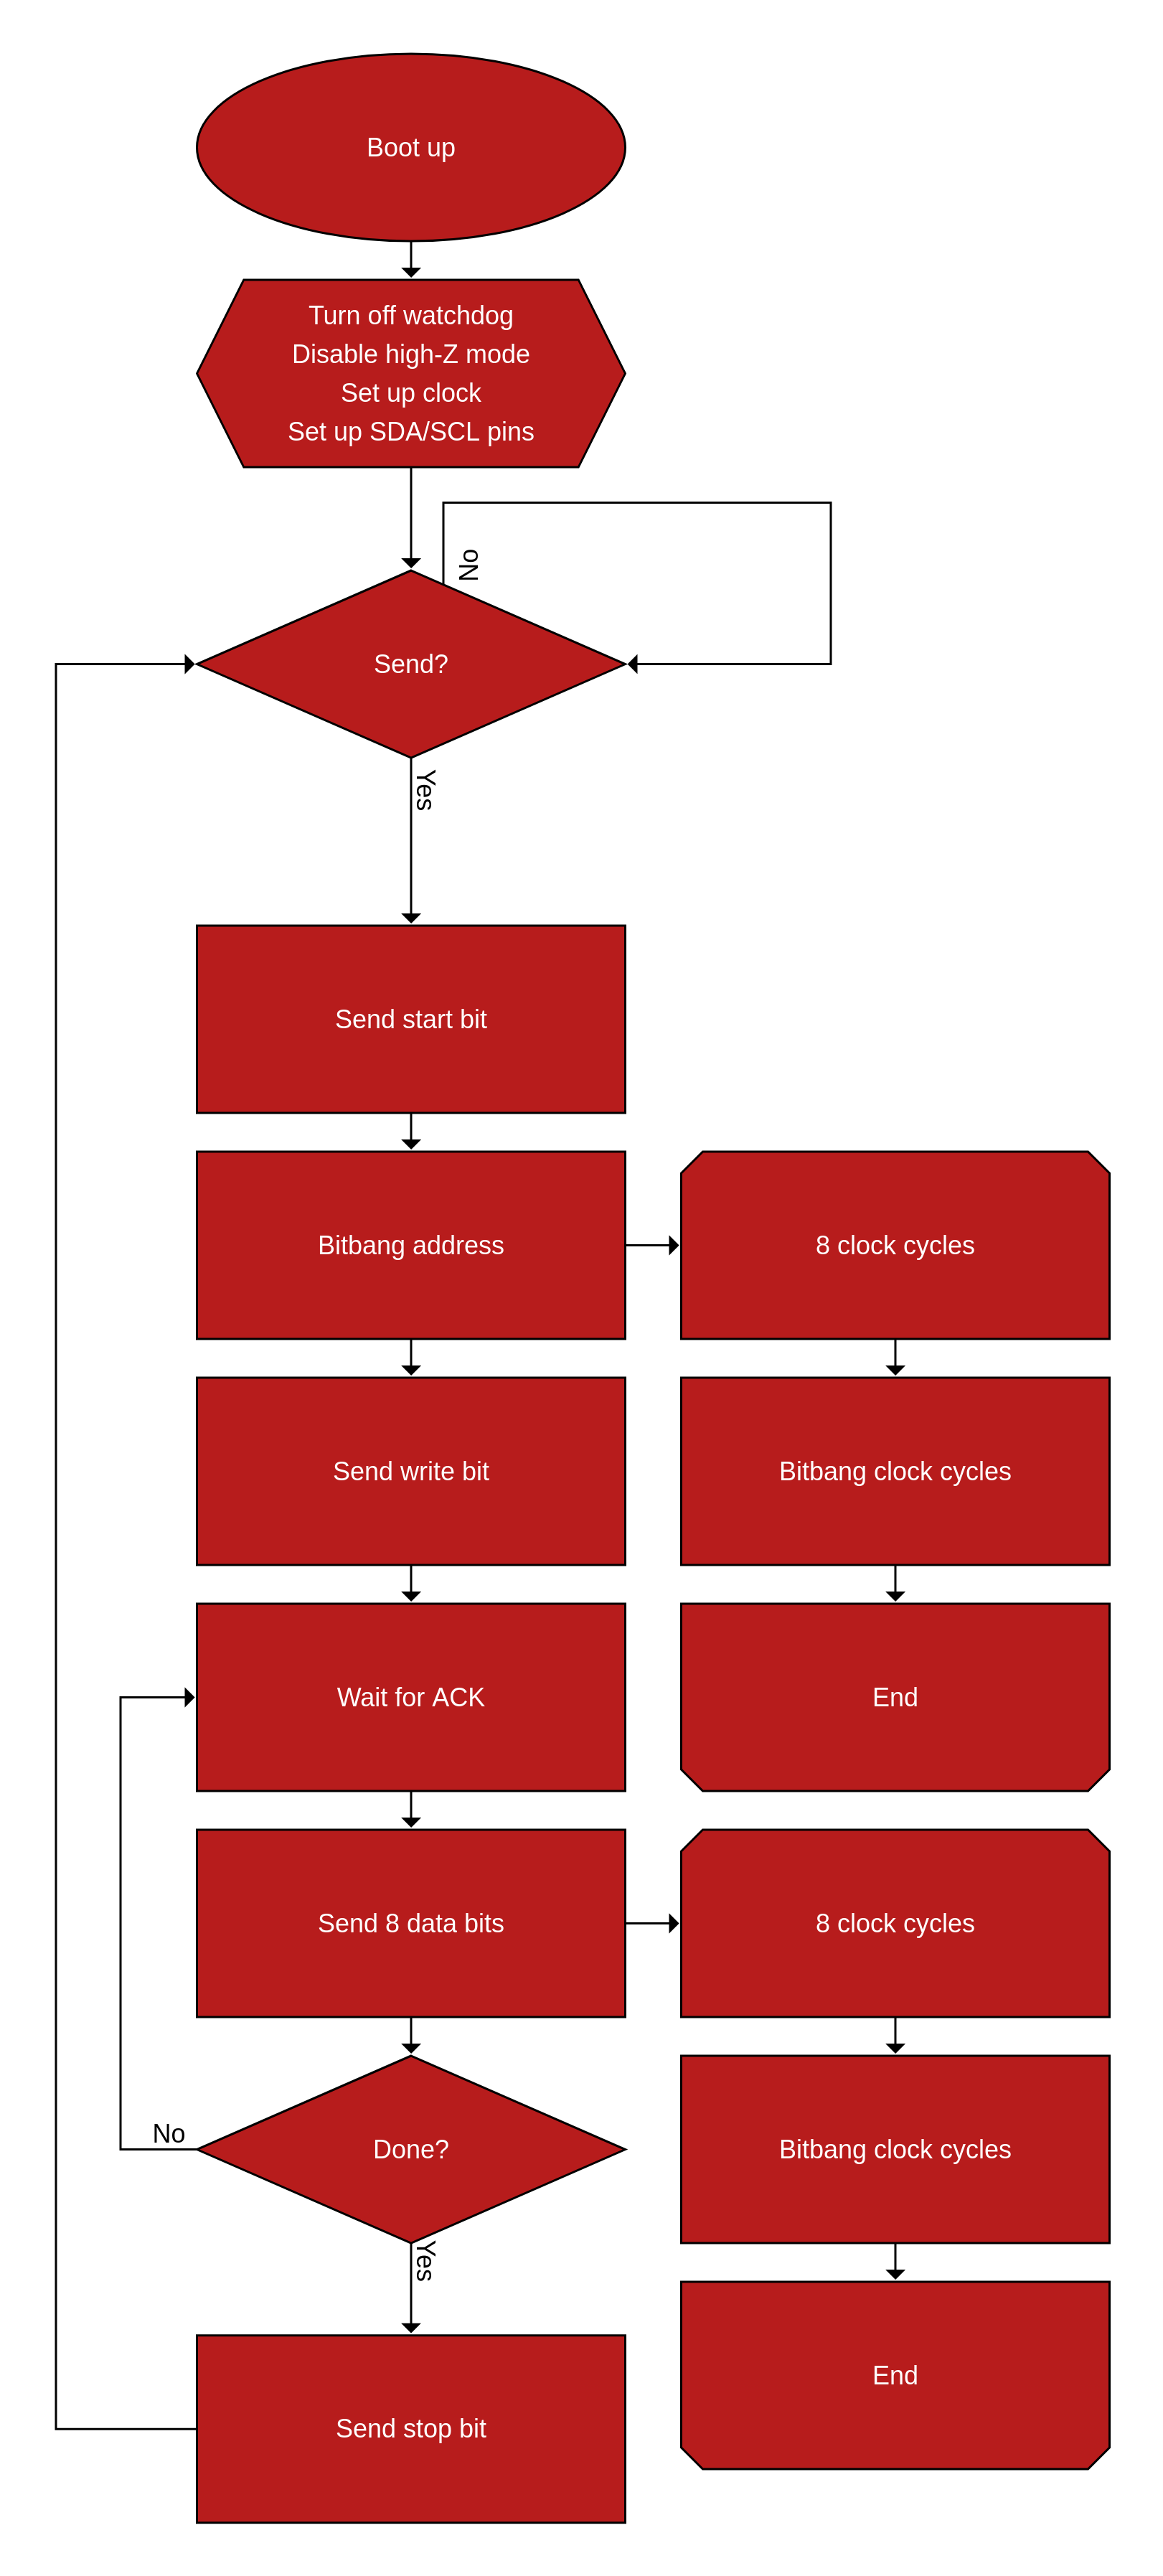
\includegraphics[width = 0.6\textwidth]{graph.png}
\captionsetup{format = hang, width = 0.75\textwidth}
\caption{Flowchart of basic I\(^2\)C writing.}
\label{fig:Flowchart}
\end{figure}
\end{centering}


%************ Bibliography ************
% \newpage
% \bibliography{Final}
% \bibliographystyle{ieeetr}
%

%--------------------------------------------------------------------------
%--------------------------------------------------------------------------
%----------------------- END DOCUMENT -------------------------------------
%--------------------------------------------------------------------------
%--------------------------------------------------------------------------
\end{document}
